\subsection{Modelování databázových systémů}
\begin{figure}[H]
	\centering
	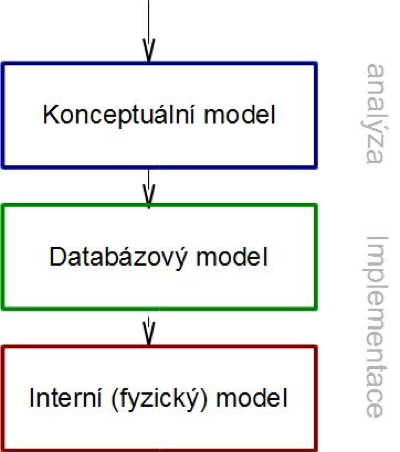
\includegraphics[width=0.3\textwidth]{assets/modelovani.png}
\end{figure}

Databázový systém můžeme modelovat \textbf{třemi datovými modely}. Ve fázi analýzy se používá \textbf{konceptuální} \textbf{model}, který modeluje realitu na logickou úroveň databáze. Konceptuální model je výsledkem datové analýzy a je \textbf{nezávislý na konkrétní implementaci}. 

V implementační fázi si pak pomáháme \textbf{databázovými} \textbf{modely}, kde modelujeme vazby a vztahy (realitu) na konkrétní tabulky (obecně SŘBD). Databázový model můžeme dále dělit na \textbf{relační} a \textbf{síťový} model. \textbf{Fyzickým uložením dat} na paměťové médium se zabývá \textbf{interní} \textbf{model}.

\subsubsection{Základní pojmy}
\begin{itemize}
	\item \textbf{Entita} -- objekt reálného světa, konkrétní výskyt instance entitního typu
	\item \textbf{Entitní typ} -- něco jako třída, je popsán jménem a množinou atribitů.
	\item \textbf{Atribut} -- vlastnost entity (možné hodnoty jsou označeny jako \textbf{doména atributu}).
	\item \textbf{Klíč} -- množina atributů, která jednoznačne určuje \textbf{entitu}.
	\item \textbf{Vztah/vazba} -- definován názvem a vztahem mezi \textbf{dvěma entitními} typy.
	\item \textbf{Kardinalita vztahu} -- dělení vztahů podle počtu entit vstupujících do vztahu -- 1:1, 1:N, M:N.
	\item \textbf{Povinnost v členství} -- musí li vztah mezi dvěma entitami existovat, či nemusí.
\end{itemize}

\subsection{Datová analýza a konceptuální model}
Datová analýza \textbf{zkoumá objekty reálného světa, jejich vlastnosti a vztahy}. Zabývá se strukturou obsahové části systému (\textbf{strukturou databaze}). Výsledkem datové analýzy je \textbf{konceptuální model}. V rámci datové analýzy zpracováváme zadání (specifikaci požadavků na IS):

\begin{itemize}
\item podtrhneme \textbf{podstatná jména} = identifikujeme \textbf{objekty},
\item podtrhneme \textbf{slovesa} = identifikujeme \textbf{vazby} mezi objekty,
\item najdeme \textbf{vlastnosti} a \textbf{stavy} nalezených objektu = identifikujeme \textbf{atributy}.
\end{itemize}

Z takto získaných informací sestavíme konceptuální model. \textbf{Konceptuální model} je jednoduchý \textbf{popis entit a jejich vzájemných vztahů}. Jedná se o jakýsi prvotní jednoduchý návrh námi vytvářené databáze. Je kladen důraz na zobrazení všech entit, jejich vztahů a je \textbf{nezávislý} na SŘBD. Skládá z:
\begin{itemize}
\item \textbf{ER Diagram}, lineární zápis \textbf{entit}, lineární zápis \textbf{vztahů}, \textbf{datový slovník}, popis dalších IO (\textbf{integritních omezení}).
\end{itemize}

\subsubsection{ER (Entity-Relationship) Diagram}
Grafické znázornění \textbf{konceptuálního modelu} (objektů a vztahů mezi nimi). Může mít několik podob v závislosti na používaném prostředí a detailnosti s jakou jej potřebujeme vypracovat. \textbf{Atributy} můžou být v grafu znázorněny \textbf{ovály} spojenými s \textbf{objekty} (\textbf{obdélníky}), \textbf{vazba} 1:N může být znázorněna ,,hráběmi'' místo N, či celý diagram se může podobat třídnímu diagramu s atributy vepsanými do objektu.

\begin{figure}[H]
	\centering
	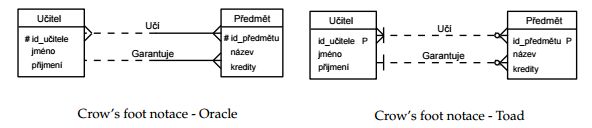
\includegraphics[width=0.7\textwidth]{assets/erdiagram.png}
\end{figure}

\textbf{Slabý entitní typ} je označení entity, která není jednoznačně definována jen svými atributy, ale i jinou entitou, se kterou je ve vztahu. Tj bez tohoto vztahu by nedávala smysl. Nejčastěji implementováno pomocí složeného primárního klíče ve slabém entitním typu, kde jeden atribut PK je rovněž cizí klíč druhé entity. V příkladu je to položka objednávky, která bez znalostí informací o objednávce nemá žádnou vypovídací schopnost.

\begin{figure}[H]
	\centering
	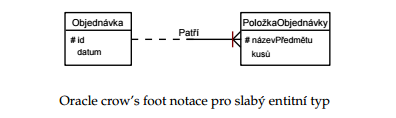
\includegraphics[width=0.7\textwidth]{assets/erdiagram_slaby_entitni_typ.png}
\end{figure}

\subsubsection{Lineární zápis entit a vztahů}
Lineárním zápisem \textbf{popisujeme objekty}, jejich vlastnosti a vztahy \textbf{z pohledu implementačního}. Lineárním zápisem entit jsou v podstatě definovány \textbf{tabulky a jejich atributy} včetně \underline{\textbf{primárních}} a \textbf{\textit{cizích klíčů}}. 

\begin{itemize}
\item Příklad lineárního zápisu entity: \texttt{Pes (\underline{IDPes}, jmeno, pohlavi, vek, CRasa, \textit{IDUtulek})}.
\item Příklad lineárního zápisu vztahů: \texttt{NABIZI (Útulek, Pes) 1:N}.
\end{itemize}

\subsubsection{Datový slovník}
\textbf{Podrobný rozpis jednotlivých atributů}. Tabulka obsahuje typ atributů, velikost, integritní omezení, atd. 

\textbf{Integritní omezení} obsahují další specifikace atributů, které nejsou dány typem a délkou. Nejčastěji se týkají formátu atributu (podmínka v jakém má být formátu) -- např: login se skládá z třech čísel a třech písmen, nebo rodné číslo je složeno z data narození, apod.

\textbf{Další integritní omezení} -- konceptuální schéma obsahuje také soupis dalších IO, které se týkají entit (tabulek) a vazeb mezi nimi. Může jít například o omezení vícenásobné vazby, vyjádření hierarchie mezi entitama, apod. 

\begin{table}[H]
	\centering
	\begin{tabular}{|l|l|l|l|l|l|}
		\hline
		\textbf{Pes} & \textbf{Typ} & \textbf{Délka} & \textbf{Klíč} & \textbf{NOT NULL} & \textbf{IO}                      \\ \hline
		IDPes        & int          & 8              & primarni      & ano               & pravidla pro tvar čipového čísla \\ \hline
		jmeno        & varchar      & 50             &               &                   &                                  \\ \hline
		rok_narozeni & int          & 4              &               &                   & Validní rok                      \\ \hline
		CRasa        & int          & 2              & sekundarni    &                   &                                  \\ \hline
	\end{tabular}
\caption{Datový slovník pro tabulku Pes.}
\end{table}

\subsection{Funkční analýza}
Zatímco datová analýza se zabývá strukturou obsahové části systému (strukturou databaze), \textbf{funkční analýza řeší funkce systému}. Funkční analýza tedy vyhodnocuje manipulaci s daty v systému. Skrze \textbf{DFD} (Data Flow Diagramy) \textbf{analyzuje toky dat}, \textbf{základní funkce systému a aktéry}, kteří se systémem pracují. Výstupem jsou pak \textbf{minispecifikace} -- podrobné analýzy elementárních funkcí systému. 

Cílem je popsat vytvářený systém jako „černou skříňku“, definovat její \textbf{vnější chování} a strukturalizovat \textbf{okolí systému}, které se systémem komunikuje. \textbf{Popsat všechny funkce, které se budou s daty provádět.}

\subsubsection*{Otázky na požadavky}
\begin{itemize}
\item\textbf{PROČ} nový systém. 
\item\textbf{ČEMU} má sloužit. 
\item\textbf{KDO} s ním pracuje - běžně, příležitostně, pravidelně zřídka. 
\item\textbf{VSTUPY} – objekty, atributy 
\item\textbf{VÝSTUPY} – výstupní sestavy, požadované informace 
\item\textbf{FUNKCE} – jaké výpočty, odvozování, výběry, třídění, \ldots
\item\textbf{Vazby na OKOLÍ systému} – odkud data a kam.
\end{itemize}

\subsubsection*{Nefunkční požadavky}
\begin{itemize}
\item Požadavky na \textbf{výsledný program}.
\item \textbf{Vnější požadavky}: ostatní nefunkční implementační požadavky, použití \textbf{standardů}, \textbf{cenová} omezení, \textbf{časové} požadavky.
\end{itemize}

\subsubsection{Diagram datových toků (DFD)}
DFD je grafický nástroj pro \textbf{modelování funkcí a vztahů v systému}. Znázorňuje nejen procesy (funkce) a datové toky, ke kterým v systému dochází, ale definuje také hlavní aktéry a jejích omezení nad systémem. DFD diagram obsahuje tyto prvky: \textbf{aktér} (obdélník mimo systém), \textbf{proces} (kruh uvnitř systému), \textbf{datové toky} (šipky) a \textbf{paměť} (viz. obr. Akce a Člen).

\begin{figure}[H]
	\centering
	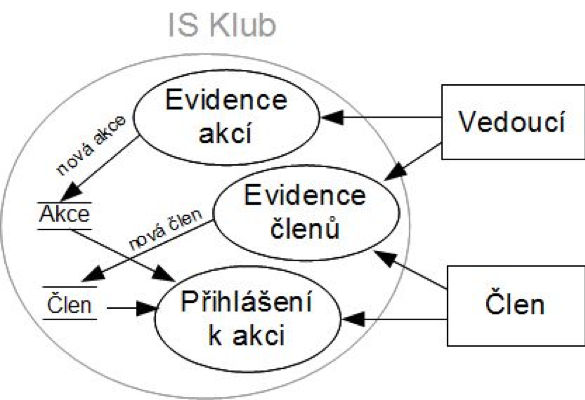
\includegraphics[width=0.4\textwidth]{assets/dfd.png}
\end{figure}

DFD diagramy lze zakreslit v různých úrovních. Např. proces Evidence akcí na obrázku lze dále rozkreslit dalším DFD, obsahující procesy vytvoření a editace akce. DFD nejvyšší úrovně se nazývá \textbf{kontextový diagram}. Znázorňuje pouze práci aktérů se systémem jako celkem. Systém v kontextovém diagramu vystupuje jako černá skříňka a v diagramu tedy nejsou použity prvky procesu a paměti.
\textbf{Hlavní znaky DFD:}

\begin{itemize}
\item Má několik úrovní podrobnosti.
\item Definuje \textbf{hranici systému}.
\item Definuje \textbf{všechny akce}, které mezi systémem a jeho okolím probíhají.
\end{itemize}

\subsubsection{Minispecifikace = algoritmy elementárních funkcí}
\begin{itemize}
\item Popisuje logiku každé z funkcí \textbf{poslední úrovně DFD}.
\item Každému \textbf{elementárnímu (nerozložitelnému) procesu} z poslední úrovně DFD odpovídá \textbf{jedna minispecifikace}.
\item Popisuje postup, jak jsou \textbf{vstupní data transformována na výstupní}.
\item Popisuje, co \textbf{funkce znamená}, ne jak se to spočítá.
\item Používá se \textbf{přirozený jazyk} s omezeným množstvím jasně definovaných pojmů, aby byla \textbf{srozumitelná} jak pro analytika, tak i uživatele a programátorovi.
\end{itemize}

\smallskip
\begin{minted}[tabsize=4,obeytabs]{sql}
IF všechny výrobky v objednávce jsou rezervovány,
THEN pošli objednávku k dalšímu zpracování oddělení prodeje.
OTHERWISE,
	FOR EVERY nezarezervovaný výrobek v objednávce DO:
		Zkus najít volný výrobek a rezervuj ho.
		IF výrobek není na skladě,
		THEN informuj správce.
\end{minted}